\documentclass[12pt, twoside]{article}
\usepackage[francais]{babel}
\usepackage[T1]{fontenc}
\usepackage[latin1]{inputenc}
\usepackage[left=5mm, right=5mm, top=5mm, bottom=5mm]{geometry}
\usepackage{float}
\usepackage{graphicx}
\usepackage{array}
\usepackage{multirow}
\usepackage{amsmath,amssymb,mathrsfs} 
\usepackage{soul}
\usepackage{textcomp}
\usepackage{eurosym}
\usepackage{lscape}
 \usepackage{variations}
\usepackage{tabvar}
 
\pagestyle{empty}


\date{}

\begin{document}

\enskip


\begin{center}
\LARGE{\ul{\textbf{Droites parall�les}}}
\end{center}

\vspace{1cm}


\section{Montrer que des droites ne sont pas parall�les}


\fbox{
\begin{minipage}{18cm}
\ul{Cons�quence du th�or�me de Thal�s}: 

\enskip





\begin{enumerate}
  \item [$\bullet$](d) et (d') sont deux droites s�cantes en A.
  \item  [$\bullet$] B et M sont deux points de (d) distincts de A.
  \item [$\bullet$] C et N sont deux points de (d') distincts de A.
\end{enumerate}


\enskip

Si deux des rapports $\dfrac{AM}{AB}$; $\dfrac{AN}{AC}$; $\dfrac{MN}{BC}$ sont
diff�rents alors les droites (BC) et (MN) ne sont pas parall�les.



\end{minipage}
}


\bigskip

\ul{M�thode pour montrer que des droites ne sont pas parall�les}:

\begin{center}
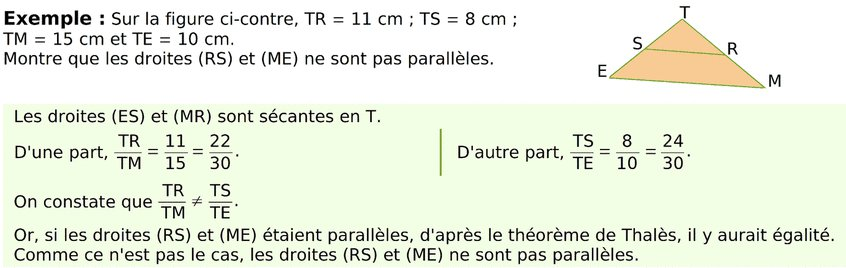
\includegraphics[width=14cm]{images/ex1.jpg}
\end{center}





\section{Montrer que des droites sont parall�les}

 

\fbox{
\begin{minipage}{18cm}
\ul{R�ciproque du th�or�me de Thal�s}: 

\enskip





\begin{enumerate}
  \item [$\bullet$](d) et (d') sont deux droites s�cantes en A.
  \item  [$\bullet$] B et M sont deux points de (d) distincts de A.
  \item [$\bullet$] C et N sont deux points de (d') distincts de A.
\end{enumerate}

 
\enskip

Si deux des rapports $\dfrac{AM}{AB}=\dfrac{AN}{AC}$ et si les points A,B et M
et les points A, N et C sont align�s dans le m�me ordre alors les droites (BC)
et (MN) ne sont pas parall�les.



\end{minipage}
}

\bigskip

\ul{M�thode pour montrer que des droites sont parall�les}:


\begin{tabular}{cc}
\begin{minipage}{15cm}
A l'aide des donn�es de la figure, montrer que les droites (AL) et (HT) sont
parall�les.
\end{minipage}
&
\begin{minipage}{4cm}
\begin{center}
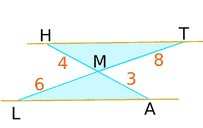
\includegraphics[width=3cm]{images/ex2.jpg}
\end{center}
\end{minipage}
\end{tabular}




\begin{itemize}
\item [$\bullet$] Les droites (AH) et (TL) sont s�cantes en M.

\item [$\bullet$] Les points A, M, H et L, M , T sont align�s dans le m�me
ordre.

\item [$\bullet$]  $\dfrac{MH}{MA}=\dfrac{4}{3}$ \quad et \quad
$\dfrac{MT}{ML}=\dfrac{8}{6}=\dfrac{4}{3}$ \qquad On constate que
$\dfrac{MH}{MA}=\dfrac{MT}{ML}$.





\end{itemize}

\enskip


Donc d'apr�s la r�ciproque du th�or�me de Thal�s, les droites (AL) et (HT) sont
parall�les.


\bigskip


\ul{Remarques}:

\enskip


\begin{itemize}
  \item [$\bullet$] Attention, il ne suffit pas de v�rifier l'�galit� des
  rapports: il faut aussi s'assurer que les points sont bien plac�s dans le
  m�me  ordre.
  \item [$\bullet$] Il ne faut pas utiliser des valeurs approch�es pour
  affirmer que deux quotients sont �gaux.
\end{itemize}

\end{document}
